\documentclass[12pt]{article}

\usepackage[utf8]{inputenc}
\usepackage{latexsym,amsfonts,amssymb,amsthm,amsmath}
\usepackage{graphicx}
\usepackage{titling}
\usepackage{gensymb}

\setlength{\parindent}{0in}
\setlength{\oddsidemargin}{0in}
\setlength{\textwidth}{6.5in}
\setlength{\textheight}{8.8in}
\setlength{\topmargin}{0in}
\setlength{\headheight}{18pt}  
\setlength{\headsep}{-30pt}
\newcommand{\overbar}[1]{\mkern 1.5mu\overline{\mkern-1.5mu#1\mkern-1.5mu}\mkern 1.5mu}
\author{Eric Lin and Kevin Zhou}

\setlength{\droptitle}{-4em}
\title{
\includegraphics[width=10cm]{Bur Oak Math Club Banner Bold.png}\\\vspace{0.25in} Gr.9-10 Class 1 Homework (Triangles)}

\begin{document}
\maketitle

\subsection*{Exercise 1}
In the figure AB = AC = CD, and AD = BD. Find the measure of $\angle$ADC in degrees.\\
\vspace*{-0.3in}
\begin{figure}[h]
    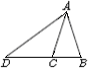
\includegraphics[scale=1.25]{image1.png}
\end{figure}

\vspace{0.50in} %Leave space for comments!

\subsection*{Exercise 2}
In the given figure, the two rectangles EFGH and ACDE share a common corner at E and overlap so
that BC = 7. What is the area of the shaded region ABGFEA?\\
\vspace*{-0.3in}
\begin{figure}[h]
    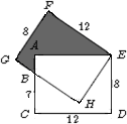
\includegraphics[scale=0.90]{image2.png}
\end{figure}

\vspace{2in} %Leave more space for comments!

\vspace{3in}

\subsection*{Exercise 3}
A square of side length S and an equilateral triangle of side length S are placed inside a rectangle of
length 2S and width S as shown. What fraction of the area of the rectangle remains uncovered?
\vspace*{-0.1in}
\begin{figure}[h]
    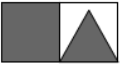
\includegraphics[scale=0.90]{image3.png}
\end{figure}

\vspace{0.5in}

\subsection*{Exercise 4}
In $\square$PQRS, M is the midpoint of PS and N is the midpoint of SR. If the area of $\triangle$SMN is 18, find the area of $\triangle$QMN.
\begin{figure}[h]
    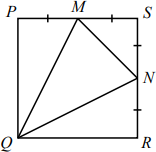
\includegraphics[scale = 0.75]{image4.png}
\end{figure}

\vspace{0.5in} %Leave space for comments!

\subsection*{Exercise 5}
The figure $\square$ABCD is a rectangle, AD = 6, AB = 18, arc AB is a semicircle with diameter AB, arc
CF is a semicircle with diameter CF, and EG is tangent to both semicircles. Find EC.\\
\vspace*{-0.3in}
\begin{figure}[h]
    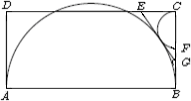
\includegraphics[]{image5.png}
\end{figure}

\vspace{0.5in} %Leave space for comments!
\vspace{3in}




\end{document}
